\documentclass[pdftex,a4paper,10pt]{article}
\usepackage{amsmath}
\usepackage{amssymb}
\usepackage{amsthm}
\usepackage{graphicx}
\usepackage{url}
\usepackage[colorlinks=true,
	linkcolor=black,
	urlcolor=black,
	pdftitle={Writing Scientific Documents Using LaTeX},
	pdfauthor={Andrew J. Bennieston}]{hyperref}

\title{Writing Scientific Documents Using \LaTeX}
\author{Andrew J. Bennieston}
\date{Fifth Edition\\
February 19, 2009}

\begin{document}
\maketitle
\tableofcontents

\section{Introduction}
\LaTeX\, is the de-facto standard for typesetting scientific documents. It is an accepted format for submission to a number of scientific journals, as well as many professional publishers. Its popularity stems from a history of flexibility, power and just `doing the right thing'. \LaTeX\, automatically numbers your equations and figures, lays content out according to strict style rules so as to obtain a readable, polished finish, and rarely gets in the way of the task of writing!

In this document, I introduce many of the \LaTeX\, commands and concepts required to produce a reasonable scientific document of any length, emphasising some of the more complicated aspects while skipping over the simpler things. In some cases, these simple things are silently included as part of a more involved example, so look closely at the example code provided!

\section{Starting a \LaTeX\, Document}
A \LaTeX\, document must have a preamble (the stuff that goes before \\
\verb|\begin{document}|). If your \LaTeX\, is split across multiple files, only the top-level file (the one from which you include the others, and run the \verb|latex| program against) needs the preamble. The preamble is where you specify the document class, include packages to provide useful functionality, and define any custom commands you need. At the very least, you must specify a document class.
\begin{verbatim}
\documentclass[10pt,a4paper]{article}
\usepackage{amsmath,amsthm,amssymb}
\end{verbatim}

The \LaTeX\, above starts a document with the \emph{article} document class. Several document classes exist, but \emph{article} serves for most purposes. Two others see some use; these are \emph{book} and \emph{report}. I generally prefer to modify the \emph{article} class to suit my purposes, since it is usually the most sensible.
The main argument to the command is enclosed in \verb|{| and \verb|}|, and arguments which are passed on to the \emph{article} class are in \verb|[| and \verb|]|. In this case, they specify to use the A4 paper size and a 10 point font. The \verb|\usepackage| command imports \LaTeX\, style files; in this case the American Mathematical Society styles, which extend and improve the mathematical typesetting provided by \LaTeX. Common packages you may want to include are listed below, with short descriptions.
\begin{description}
\item[amsmath] provides additional mathematical typesetting
\item[amssymb] provides mathematical symbols
\item[amsthm] provides theorem formatting for AMS publications
\item[fancyhdr] provides customisable headers and footers
\item[graphics] provides graphics support
\item[graphicx] provides extended graphics support (use instead of \textbf{graphics})
\item[hyperref] provides navigation support for PDF documents (clickable references, etc.)
\item[url] provides clickable URL support
\end{description}
Many of the packages listed require arguments and customisations to function correctly. Each one has online documentation which may be consulted.

The title, authors and date are also usually included in the preamble. This is achieved as follows:
\begin{verbatim}
\title{My Report}
\author{C. Turk \and J. Dorian}
\date{\today}
\end{verbatim}
The contents of those fields can be anything you like --- you could use the date field to insert a lecture number as well as a date, for example \\
\verb|\date{\today -- Lecture 2}|. If the date field is omitted, the current date will be included automatically, but explicitly stating it makes it clearer!

Finally, the document itself is started with \verb|\begin{document}| and ended with \verb|\end{document}|. The title, author and date fields are typeset with the \verb|\maketitle| command, and a table of contents can be included with the cunningly named \verb|\tableofcontents| command. A complete \LaTeX\, document template might look something like this:
\begin{verbatim}
\documentclass[12pt,a4paper]{article}
\usepackage{amsmath,amssymb,fancyhdr,url}
\usepackage[pdftex]{graphicx}

\title{My Report, Mk. II}
\author{J. Dorian \and B. Kelso}
\date{Before time began\ldots}

\begin{document}
\maketitle
\newpage
\tableofcontents
\newpage

\section{Life at Sacred Heart}
This is the story of \ldots

\end{document}
\end{verbatim}

There are a few new things introduced here; sections will be covered later, but let us briefly mention the \verb|\newpage| command, which does exactly what it says on the tin, and the \verb|\ldots| command, which produces: \ldots

\section{Sections and Subsections}
Sections are started with the \verb|\section{section-title}| command. The section title goes between the \verb|{}|. Similarly, subsections are started with the \verb|\subsection{sub-title}| command, and sub-subsections with the \\
\verb|\subsubsection| command. By default, all sections and nested subsections are automatically numbered. This behaviour can be turned off on a per-section basis by using the \verb|\section*{section-title}| form, where the \verb|*| tells \LaTeX\, not to number these sections according to the document numbering scheme. The \verb|*| can be used on (almost) anything which would normally be numbered; (sub)sections, equations, etc. Figures and tables use the \verb|*| option in a different way because their naming and numbering is controlled through the \verb|\caption| command.

\section{Typesetting Considerations}
\LaTeX\, is a little more pedantic than most word-processors, and requires certain punctuation marks to be typeset in slightly different ways. This section discusses the most commonly encountered issues.

\subsection{Single Quotes}
\LaTeX\, requires left and right quotes, rather than straight quotes. Using the apostrophe, \verb|'|, always produces a right quote, so you need to use the \emph{backtick}, \verb|`|, to obtain a left-quote. Quoted text then looks something like \emph{the `flavour' of a particle} and not like \emph{the 'flavour' of a particle}. The former produces the correct result when typeset, the latter begins and ends with end-quotes!

\subsection{Double Quotes}
Double left-quotes are input using two single left quotes (the backtick), while double right-quotes are input using two single right quotes (the apostrople). Double quoted text is typeset something like \verb|\ldots said| \verb|``the project| \verb|is on| \verb|schedule| \verb|and an| \verb|investigation has been launched''|, which looks something like this when typeset: \ldots said ``the project is on schedule and an investigation has been launched''

\subsection{An Aside on Quotation Marks}
In British English, the usual practice is to enclose quoted matter between single quotation marks, reserving double quotation marks for a quotation within a quotation. In US English, the reverse is true. For quotations nested within the second quotation, one should revert to the original mark, alternating accordingly for subsequent levels.

\subsection{Hyphenation and Dashes}
Hyphens and dashes in printed text have three sizes; the soft hyphen, used to split a word across a line, is the shortest. This is automatically inserted by \LaTeX\, when required. The hard hyphen is the same length as its soft sibling. It is used to hyphenate words within a line, and is typeset using a single dash (\verb|-| $\Rightarrow$ -). The en-rule (or en-dash) marks a range (often of numbers), such as 3--5. This is slightly longer (one \emph{en} in length), and is typeset using two hyphens (\verb|--| $\Rightarrow$ --). Finally, the em-rule (or em-dash) is used to insert a pause in text --- which should probably be replaced by a comma or semicolon anyway --- and is the longest (one \emph{em} in length). It is typeset using three hyphens (\verb|---| $\Rightarrow$ ---).

\subsection{Special Characters}
There are some characters which are used by \LaTeX\, as control sequences. These must be escaped to be used in normal text. The characters most often encoutered are \verb|\ _ & % { } #| (begin command, underscore, table separator, comment, left curly brace, right curly brace, hash or ``pound'' sign) and they can be produced in the text verbatim by `escaping' with a leading backslash: \verb| \_ \& \% \{ \} \#|, with the exception of the backslash, which can be inserted with the \verb|\textbackslash| command: \textbackslash.

\subsection{Emphasising Text}
To place emphasis on a certain phrase, use the \verb|\emph{something}| command. This usually produces \emph{italic} text, but the effect depends on the document style used. The advantage of using \verb|\emph| is that emphasised text within an already emphasised section is typeset in Roman (non-italic) text. For example, \verb|The \emph{President of | \verb|the \emph{United| \verb|States} of America}| produces: The \emph{President of the \emph{United States} of America}.

In addition, it is possible to directly specify the typeface required. The command \verb|\textit{italic text}| produces \textit{italic text}, while \verb|\textbf{bold text}| produces \textbf{bold text} and \verb|\texttt{monospaced text}| produces \texttt{monospaced text}.

\section{Mathematical Typesetting}
\LaTeX\, provides several environments for mathematics and I will not cover them all here. Instead, I will mention those which are most important in short documents and reports.

\subsection{Inline Mathematics}
To insert mathematics inline with the paragraph text you can use the \verb|$...$| environment. This is achieved as follows:
\begin{verbatim}
The solar neutrino flux was found to be
$2.1 \pm 1$ solar neutrino units (SNU).
\end{verbatim}
When typeset, this looks like: The solar neutrino flux was found to be $2.1 \pm 1$ solar neutrino units (SNU).

The use of \verb|$...$| to insert math-mode \LaTeX\, inline with the paragraph text allows for many $\epsilon$ff$\epsilon$$\hat{c}\tau$s; I used it to produce the right-arrows ($\Rightarrow$) in the hyphenation section, above.

\subsection{Display Mathematics}
The display mathematics environment sets mathematical content on a line of its own, centred on the page. The shortcut form is the \verb|\[...\]| environment, which enters display mode but does not add equation numbering.
\[ \frac{\hbar^2}{2m}\nabla^2\Psi + V(\mathbf{r})\Psi 
= -i\hbar \frac{\partial\Psi}{\partial t} \]
The Schr\"odinger equation, above, was typeset using:
\begin{verbatim}
\[ \frac{\hbar^2}{2m}\nabla^2\Psi + V(\mathbf{r})\Psi 
= -i\hbar \frac{\partial\Psi}{\partial t} \]
\end{verbatim}

To get equation numbering, one has to be slightly more verbose:
\begin{verbatim}
\begin{equation}\label{rw-metric}
ds^2 = c^2 dt^2 \left( \frac{d\sigma^2}{1-k\sigma^2}
+ \sigma^2\left[ d\theta^2 + \sin^2\theta d\phi^2 \right] \right)
\end{equation}
\end{verbatim}
\ldots which looks like:
\begin{equation}\label{rw-metric}
ds^2 = c^2 dt^2 \left( \frac{d\sigma^2}{1-k\sigma^2}
+ \sigma^2\left[ d\theta^2 + \sin^2\theta d\phi^2 \right] \right)
\end{equation}

Note that the \verb|\label| command was used here, which sets a label that can used in references to that equation. For example, typing \verb|\eqref{rw-metric}| at any point in the document will yield: \eqref{rw-metric}. As with sections, using the ``starred form'' \verb|\begin{equation*}| suppresses equation numbering (which is precisely what \verb|\[...\]| does).

\subsection{The Align Environment}
To typeset equations over multiple lines, use the \emph{align} environment, of the \emph{amsmath} package. Here is an example with the \emph{align} environment:
\begin{verbatim}
\begin{align}
X(t) = 1 + \frac{t^3}{2t} \\
= 1 + \frac{t^2}{2}
\end{align}
\end{verbatim}
\begin{align}
X(t) & = 1 + \frac{t^3}{2t} \\
& = 1 + \frac{t^2}{2}
\end{align}

The ampersand character, \&, is used to set the alignment points. Note that using the \emph{align} environment does not squash fractions into a single line height! Line numbers can be suppressed with \verb|\nonumber|, and the environment and \emph{align*} provides an unnumbered version of the same functionality.

\subsection{Symbols}
There is a lot of documentation on the \LaTeX\, mathematical command set. For the most part it is obvious; Greek letters are produced using \verb|\lettername|, for example $\gamma$ is \verb|$\gamma$|. Uppercase Greek letters are obtained by capitalising the first letter: $\Omega$ is \verb|$\Omega$|\ldots

There are also a variety of arrows and other symbols: \verb|$\rightarrow$| produces $\rightarrow$. Many more exist, and the \emph{Comprehensive \LaTeX\, Symbol List}\footnote{\url{http://www.ctan.org/tex-archive/info/symbols/comprehensive/symbols-a4.pdf}} covers a huge number of mathematical, scientific and other symbols.

Summation symbols can be inserted either with \verb|\sum| or \verb|\Sigma|, though \verb|\sum| is preferred, since it scales as required. Integrals can be represented using \verb|\int| and variants for double integration, closed loop integration, etc.
\begin{verbatim}
\[ \sum_{i=1}^N \rightarrow \int_1^N\,\mathrm{d}i \]
\end{verbatim}
\[\sum_{i=1}^N \rightarrow \int_1^N\,\mathrm{d}i\]

\subsection{Fractions}
Fractions can be typeset in the form $1/2$: \verb|$1/2$|, or with horizontal lines $\frac{1}{2}$: \verb|$\frac{1}{2}$|. Fractions and many other symbols are sized differently depending on whether the equation is inline (part of the paragraph text) or displayed. To use the display sizes for inline symbols, add the \verb|\displaystyle| command to the inline equation: \verb|$\displaystyle\frac{1}{2}$| renders: $\displaystyle\frac{1}{2}$

\subsection{Brackets}
Brackets can, for the most part, be inserted normally. To scale the bracket (in displayed equations) so that it fits around the content, use \verb|\left| and \verb|\right| before the bracket character itself; for an example see equation \eqref{rw-metric}, the Robertson-Walker metric. Angle brackets such as those used in Dirac notation can be produced with \verb|\langle| and \verb|\rangle|: \verb#$\langle\psi|\hat{H}|\psi\rangle$# produces $\langle\psi|\hat{H}|\psi\rangle$. Again, \verb|\left| and \verb|\right| can be used where necessary. In order to suppress a bracket on either the left or the right, use \verb|\left.| or \verb|\right.| to prevent \LaTeX\, complaining about unbalanced brackets.

\subsection{Differentials}
Differentials can be typeset in a number of ways. The simplest method is to use \verb|\frac{dy}{dx}|: $\frac{dy}{dx}$. Some people like the $d$ to be typeset in Roman (rather than italic) or bold font: \verb|\frac{\mathrm{d}y}{\mathrm{d}x}| or \verb|\frac{\mathbf{d}y}{\mathbf{d}x}|, producing $\frac{\mathrm{d}y}{\mathrm{d}x}$ and $\frac{\mathbf{d}y}{\mathbf{d}x}$ respectively.

Partial derivatives can be typeset using the \verb|\partial| symbol in place of the $d$: \verb|\displaystyle\frac{\partial y}{\partial x}| which gives $\displaystyle\frac{\partial y}{\partial x}$. The various vector differentials can be typeset using \verb|\nabla| and decorations: $\nabla^2$, $\nabla\times\mathbf{A}$.

\subsection{Matrices}
The \emph{array} environment, used within one of the mathematical environments, can be used to typeset row and column vectors, matrices, lists of equations, etc. One must specify a column alignment for each column in the array, then use it just as the \emph{eqnarray} environment:
\begin{verbatim}
\begin{equation}
\mathbf{V}_{CKM} = \left(
	\begin{array}{ccc}
	V_{ud} & V_{us} & V_{ub} \\
	V_{cd} & V_{cs} & V_{cb} \\
	V_{td} & V_{ts} & V_{tb}
	\end{array}
\right)
\end{equation}
\end{verbatim}
\begin{equation}
\mathbf{V}_{CKM} = \left(
	\begin{array}{ccc}
	V_{ud} & V_{us} & V_{ub} \\
	V_{cd} & V_{cs} & V_{cb} \\
	V_{td} & V_{ts} & V_{tb}
	\end{array}
\right)
\end{equation}

Determinants can be typeset in a similar way by using \verb|\left\vert| and \verb|\right\vert|:
\begin{equation}
\mathrm{det~} \mathbf{I} = \left\vert
	\begin{array}{ccc}
	1 & 0 & 0 \\
	0 & 1 & 0 \\
	0 & 0 & 1
	\end{array}
\right\vert = 1
\end{equation}

To omit the brackets on one side, use \verb|\left.| or \verb|\right.|:
\begin{verbatim}
\begin{equation}\label{sim-eq}
\left.
\begin{array}{c}
x + y = 3 \\
x^2 + y = 5
\end{array}\right\} \Rightarrow x=2~,~y=1
\end{equation}
\end{verbatim}
\begin{equation}\label{sim-eq}
\left.
\begin{array}{c}
x + y = 3 \\
x^2 + y = 5
\end{array}\right\} \Rightarrow x=2~,~y=1
\end{equation}

\subsection{Math-mode Spacing}
It is possible to add spaces of varying lengths to your mathematical typesetting. In the simultaneous equations example, equation \eqref{sim-eq}, I used \verb|~,~| to add spaces either side of the comma. I also typeset integrals using \verb|\int f(x)\,dx|, where the \verb|\,| adds a small space before the $dx$ symbol:
\begin{verbatim}
\[\langle\psi|\psi\rangle = 
\int_{-\infty}^{\infty} \psi^\star(x)\psi(x) \, dx\]
\end{verbatim}
\[\langle\psi|\psi\rangle = 
\int_{-\infty}^{\infty} \psi^\star(x)\psi(x) \, dx\]

\section{Graphics}
Graphics can be inserted into \LaTeX\, documents from a number of formats. Depending on whether you use \verb|latex| or \verb|pdflatex|, the recommended formats are Encapsulated PostScript (EPS) and Portable Document Format (PDF), respectively. These formats are good because they are scalable, though non-scalable bitmap formats are supported, including JPEG. The \emph{graphicx} environment allows inclusion of such graphics, as well as modification in-place (rotating, scaling, etc.) Full documentation for \emph{graphicx} is available online.\footnote{\url{http://www.ctan.org/tex-archive/macros/latex/required/graphics/grfguide.pdf}}

\begin{verbatim}
\begin{figure}
\centering
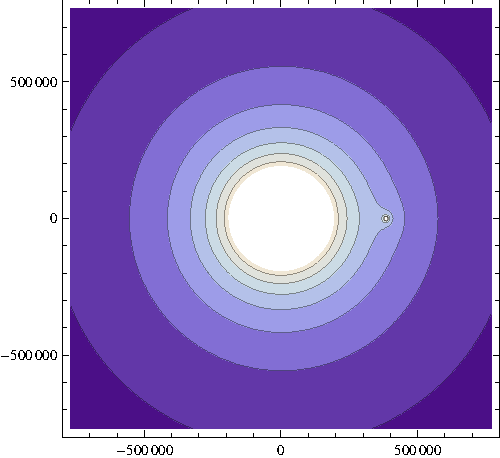
\includegraphics[scale=0.75]{earth-moon.pdf}
\caption{\label{earth-moon}The combined gravitational
potentials of the Earth and Moon.}
\end{figure}
\end{verbatim}
\begin{figure}
\centering
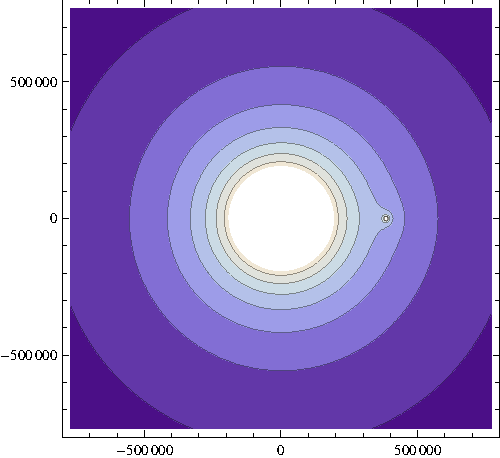
\includegraphics[scale=0.75]{earth-moon.pdf}
\caption{\label{earth-moon}The combined gravitational potentials of the Earth and Moon.}
\end{figure}

The \verb|\centering| command causes the contents of the figure to be centred (horizontally) on the page. The \verb|\label| command is used to create a reference to the figure so that we can later refer to it in the text using the command \verb|Figure \ref{earth-moon}|, i.e. Figure \ref{earth-moon}. Note also that the command \verb|\includegraphics| takes arguments which allow us to manipulate the image; here we've scaled it to 75\% of its original size. The \verb|\caption| command should be fairly self-explanatory!

Note that this document was produced using the \emph{graphicx} package; the \emph{graphics} package requires scaling and rotating to be done in a different way, but since almost all sites now have the \emph{graphicx} package installed, I'm going to ignore the \emph{graphics} package here.

\LaTeX\, will try to position graphics on a page according to a set of rules about the minimum number of lines of text on a page, and other typographic concerns. If it cannot satisfy all of these requirements the figure will be placed on a page of its own. It is possible to provide \LaTeX\, with hints for positioning a figure, given as options to the \emph{figure} environment. The hint is provided in square brackets after the environment is opened, for example \verb|\begin{figure}[t]| to request that a figure is placed at the top of a page. The following placement specifiers are understood by \LaTeX:
\begin{description}
\item[h] places the floating figure approximately at the point it occurs in the source text.
\item[t] places the floating figure at the top of the page.
\item[b] places the floating figure at the bottom of the page.
\item[p] places the figure on a special page for floated items only.
\item[!] overrides \LaTeX\, rules for determining figure positions.
\item[H] places the floating figure at precisely the point it occurs in the source text, and requires the \emph{float} package.
\end{description}

\section{Tables}
To insert a table into a \LaTeX\, document, you must enter the \emph{table} environment, then define your table as required, using the \emph{tabular} environment!

\begin{verbatim}
\begin{table}
\centering
\begin{tabular}{|c|c|}
\hline
Natural & $\mathbb{N}$ \\
\hline
Integer & $\mathbb{Z}$ \\
\hline
Real & $\mathbb{R}$ \\
\hline
Rational & $\mathbb{Q}$ \\
\hline
Complex & $\mathbb{C}$ \\
\hline
\end{tabular}
\caption{\label{my-table}A table!}
\end{table}
\end{verbatim}

\begin{table}
\centering
\begin{tabular}{|c|c|}
\hline
Natural & $\mathbb{N}$ \\
\hline
Integer & $\mathbb{Z}$ \\
\hline
Real & $\mathbb{R}$ \\
\hline
Rational & $\mathbb{Q}$ \\
\hline
Complex & $\mathbb{C}$ \\
\hline
\end{tabular}
\caption{\label{my-table}A table!}
\end{table}

The \emph{tabular} environment acts much like the \emph{array} math environment, and the \verb#|# character instructs \LaTeX\, to draw a vertical line between columns. You can use the \verb|\hline| command to draw horizontal lines. Such a table can, of course, be referred to using the \verb|\ref{my-table}| command: table \ref{my-table}.

The \emph{booktabs}\footnote{\url{ftp://ftp.tex.ac.uk/tex-archive/macros/latex/contrib/booktabs/booktabs.pdf}} package documentation includes a number of points for correctly typesetting tables, particularly for professional book layouts.

\section{Including \LaTeX\, Files}
If your document is split across several files, they can be included with the command \verb|\include{filename}|. The \verb|.tex| extension is not required --- \LaTeX\, adds it automatically. \verb|\include| will add a page-break before the contents of the included file.

The \verb|\include| command will not work inside a file which has already been \verb|\include|d by another file. The \verb|\input| command is also useful.

\section{Bibliographies \& Citations}
\subsection{Bibliographies \& References}
A simple bibliography can be created as follows:
\begin{verbatim}
\begin{thebibliography}{99}
\bibitem{Fey49} R. P. Feynman,
Space-Time Approach to Quantum Electrodynamics,
Phys. Rev. \textbf{76} 6 (1949)
\bibitem{Cas48} H. B. Casimir, On the attraction
between two perfectly conducting plates,
Proc. K. Ned. Akad. Wetensch. \textbf{51} (1948)
\end{thebibliography}
\end{verbatim}

The \verb|{99}| tells \LaTeX\, how many digits to reserve for bibliography reference numbers --- twi, in this case. If you have over 100 references, use a three-digit number.

The section title will depend on the document class used; in the \emph{article} class, it is `References', in the \emph{book} or \emph{report} class, it is `Bibliography'. You can use \verb|\begin{thebibliography*}| to suppress a title and use your own.

\subsection{Citations}
Citing bibliography items is achieved through the use of the \verb|\cite{label}| command. This adds the corresponding reference number in square brackets, at that point in the text.

\subsection{Bib\TeX}
For more complicated bibliographies, or larger documents, the Bib\TeX\, system allows a lot more flexibility and control over the presentation of bibliographic items. Documentation is available online.\footnote{\url{http://www.bibtex.org/}}

\section{Processing \LaTeX\, Documents}
Once a \LaTeX\, document has been written, it must be processed by \LaTeX\, to produce a file in the required format (e.g. DVI, PDF, PS). I prefer the \verb|pdflatex| command, which produces PDF output directly, and supports hyperlinked PDFs, where the relevant packages (\emph{url} and \emph{hyperref}) have been used.

The \verb|pdflatex| command should be run at least twice, since \LaTeX\, passes through once, enumerating the sections, equations, figures, tables and references, then the second run substitutes in the correct numbers at each point they are referenced. In this way, \LaTeX\, is able to produce the correct number for references which have not been defined prior to their point of use (e.g. bibliography items and forward-references to figures or equations). The command I run is usually something like the one below, for a file called \verb|report.tex|
\begin{verbatim}
pdflatex report && pdflatex report && pdflatex report
\end{verbatim}

It is possible to create a DVI file by processing the document with the \verb|latex| command. Again, you need to run \LaTeX\, twice or more to get all of the correct references, and a DVI can be converted to PostScript or PDF using \verb|dvips| or \verb|dvipdf|. Directly producing PDF through the \verb|pdflatex| command is, however, my preferred method.

A final point about processing the documents is that Bib\TeX\, requires the \verb|bibtex| command to be run between calls to \verb|pdflatex| (or just \verb|latex|). I put it after the first call to \verb|pdflatex|:
\begin{verbatim}
pdflatex report && bibtex report && 
pdflatex report && pdflatex report
\end{verbatim}

\section{About This Document}
This document is copyright \copyright\, 2007--2009 Andrew J. Bennieston. It may be freely distributed according to the terms of the LaTeX Project Public License (details below). The document was produced in the Vim text editor on the OpenSUSE Linux operating system. Earlier versions were produced on an Apple Macbook using the TextMate text editor, and the Slackware Linux operating system using the Vim text editor.

\subsection{License}
This work may be distributed and/or modified under the conditions of the LaTeX Project Public License, either version 1.3 of this license or (at your option) any later version. The latest version of this license is in \url{http://www.latex-project.org/lppl.txt} and version 1.3 or later is part of all distributions of LaTeX version 2005/12/01 or later.

This work has the LPPL maintenance status `maintained'. The Current Maintainer of this work is Andrew J. Bennieston. This work consists of the files scidoc.tex, Makefile, README, earth-moon.pdf and the derived file scidoc.pdf.

\subsection{History}
\begin{itemize}
\item First Edition: February 4, 2007
\item Second Edition: March 8, 2007
\item Third Edition: June 13, 2008
\item Fourth Edition: September 13, 2008
	\begin{itemize}
		\item Licence changed to LPPL (September 16, 2008).
	\end{itemize}
\item Fifth Edition: February 18, 2009
	\begin{itemize}
		\item Minor corrections (February 19, 2009)
	\end{itemize}
\end{itemize}

\end{document}
